\documentclass{beamer}

\usepackage[utf8]{inputenc}
\usepackage[russian]{babel}

\usepackage{graphicx}
\usepackage{gensymb}

\usefonttheme[onlymath]{serif}

%\usepackage{beamerthemesplit}
%\useoutertheme{infolines}
%\useoutertheme{smoothtree}
\useoutertheme{tree}
\useinnertheme{circles}
\setbeamertemplate{itemize items}[default]
\setbeamertemplate{enumerate items}[default]

\definecolor{myblue}{rgb}{.0,.2,.3}
\setbeamercolor*{palette primary}{use=structure,fg=white,bg=myblue}
\setbeamertemplate{navigation symbols}{}

\usepackage{tikz}
\usetikzlibrary{shapes.geometric, arrows, trees}
\tikzstyle{every node}=[font=\tiny, node distance=0.8cm]
\tikzstyle{io} = [trapezium, trapezium left angle=70, trapezium right angle=110, minimum width=1cm, minimum height=0.33cm, text centered, text width=1cm, draw=black, fill=blue!30]
\tikzstyle{process} = [rectangle, minimum width=1cm, minimum height=0.31cm, text centered, draw=black, fill=orange!30]
\tikzstyle{decision} = [diamond, minimum width=1cm, minimum height=0.31cm, text centered, draw=black, fill=green!30]
\tikzstyle{arrow} = [thick,->,>=stealth]
\tikzstyle{bigrect} = [rectangle, minimum width=5.5cm, minimum height=4.5cm, text depth=5cm, draw=black, dashed]

%\usepackage{verbatim}
\usepackage{listings}
%\usepackage{enumitem}
%\setlistdepth{9}
%\setlist[itemize,1]{label=$\bullet$}
%\setlist[itemize,2]{label=$\bullet$}
%\setlist[itemize,3]{label=$\bullet$}
%\setlist[itemize,4]{label=$\bullet$}
%\setlist[itemize,5]{label=$\bullet$}
%\setlist[itemize,6]{label=$\bullet$}
%\setlist[itemize,7]{label=$\bullet$}
%\setlist[itemize,8]{label=$\bullet$}
%\setlist[itemize,9]{label=$\bullet$}
%\renewlist{itemize}{itemize}{9}

\newcommand{\layersInRealLife} {
  \frametitle{Уровни (levels / layers) в реальной жизни}
  \framesubtitle{Уровни характеризуются \textbf{обязанностями} и определяют \textbf{кто над кем главнее (выше)}}

  \begin{itemize}
    \item Директор конторы (высокий уровень)
      \begin{itemize}
        \item Художник (низкий уровень)
        \item Программист (низкий уровень)
        \begin{itemize}
          \item Младший программист (самый низкий уровень)
        \end{itemize}
      \end{itemize}
  \end{itemize}
}

\newcommand{\paradigmsImpDecl} {
  \node (imper) [bigrect, xshift=-1cm] {Императивное};
  \node (decl) [bigrect, xshift=5cm, yshift=2.5cm] {Декларативное};
}

\newcommand{\paradigmsAlg} {
  \paradigmsImpDecl

  \node (alg) [process, dashed, xshift=-1cm, yshift=1cm] {Алгоритмическое};
    \node [xshift=-1cm, yshift=0.65cm] {Блок-схемы, словесное описание};
}

\newcommand{\paradigmsStruct} {
  \paradigmsAlg

  \node (struct) [process, xshift=0cm, yshift=0cm] {Структурное};
    \node [xshift=0cm, yshift=-0.35cm] {Ограничение алгоритмического};
  \draw [arrow] (alg) -- (struct);
}

\newcommand{\paradigmsProc} {
  \paradigmsStruct

  \node (proc) [process, xshift=-1cm, yshift=-1cm] {Процедурное};
    \node [xshift=-1cm, yshift=-1.35cm] {C, Pascal...};
  \draw [arrow] (struct) -- (proc);
}

\newcommand{\paradigmsOop} {
  \paradigmsProc

  \node (oop) [process, xshift=-1.5cm, yshift=-2cm] {Объектно-ориентированное (ООП)};
    \node [xshift=-1.5cm, yshift=-2.35cm] {C++, C\#, Java, Python, Ruby, JS, ...};
  \draw [arrow] (proc) -- (oop);
}

\newcommand{\paradigmsDecls} {
  \paradigmsOop

  \node (notprog) [process, dashed, xshift=5cm, yshift=4cm] {Описания};
    \node [xshift=5cm, yshift=3.65cm] {Конфигурации и Web API (XML, JSON),};
    \node [xshift=5cm, yshift=3.35cm] {вёрстка (HTML, LaTeX), аннотации};
}

\newcommand{\paradigmsFunc} {
  \paradigmsDecls

  \node (func) [process, xshift=4cm, yshift=2.5cm] {Функциональное};
}

\newcommand{\paradigmsLogical} {
  \paradigmsFunc

  \node (logical) [process, xshift=5cm, yshift=1cm] {Логическое};
}

\newcommand{\paradigmsAll} {
  \paradigmsLogical

  \node (generic) [process, xshift=-1cm, yshift=5cm] {Обобщенное};
  \node (concurrent) [process, xshift=5cm, yshift=-2cm] {Конкурентное};
  \node (module) [process, xshift=-2cm, yshift=4cm] {Модульное};
}


\title{Введение в программирование}
\author{Лопатин Александр}
\date{2015}


\subtitle{Лекция 3}

\begin{document}

  \frame{\titlepage}


  \section*{Содержание} {
    \frame{\tableofcontents[hideallsubsections]}


  \section{Способы испортить структуру}
    \frame {
      \frametitle{Способы испортить структуру}
      Способы испортить структуру программы:

      \begin{itemize}
        \item безусловный переход \textbf{goto} --- большое зло, особенно в кривых руках
          \begin{itemize}
            \item большинство программистов \underline{обязуются не использовать} этот оператор
            \item оператор популярен в низкоуровневой разработке (драйвера устройств, etc.) для обработки ошибок
            \item во многих современных высокоуровневых языках этот оператор \underline{отсутствует}
          \end{itemize}
        \item (спорно) \textbf{break} и \textbf{continue}
        \item (спорно) внезапный \textbf{return}
        \item неправильное использование \textbf{switch}/\textbf{case}/\textbf{break}
      \end{itemize}
    }

\begin{frame}[fragile]
  \frametitle{break и continue --- синтаксический сахар (Java)}
  \framesubtitle{continue}
  \begin{minted}{java}
while (i < 0) {
    if (a) {
        continue;
    }
    b();
    i = i + 1;
}
  \end{minted}
тоже самое, что и
  \begin{minted}{java}
while (i < 0) {
    if (!a) {
        b();
    }
    i = i + 1;
}
  \end{minted}
\end{frame}

\begin{frame}[fragile]
  \frametitle{break и continue --- синтаксический сахар (Java)}
  \framesubtitle{break}
  \begin{minted}{java}
while (i < 0) {
    if (a) {
        break;
    }
    b();
    i = i + 1;
}
  \end{minted}
тоже самое, что и
  \begin{minted}{java}
while (i < 0 && !a) {
    b();
    i = i + 1;
}
  \end{minted}

  \textbf{В простых случаях} ничего break и continue не портят

  Можно использовать, если добавляют выразительности в код
\end{frame}

\begin{frame}[fragile]
  \frametitle{Внезапный return}
  \begin{minted}{java}
int f(int x) {
    if (x < 0) {
        return -1;
    }

    int y = blabla(x);
    return y;
}
  \end{minted}

тоже самое, что и ...
\end{frame}

\begin{frame}[fragile]
  \frametitle{Внезапный return}
  \begin{minted}{java}
int f(int x) {
    if (x < 0) {
        return -1;
    } else {
        int y = blabla(x);
        return y;
    }
}
  \end{minted}

  Оба варианта нормальные, но второй предпочтительней
\end{frame}

\begin{frame}[fragile]
  \frametitle{Неправильное использование \textbf{switch}/\textbf{case}/\textbf{break}}
Пусть
  \begin{minted}{java}
final int READY = 1;
final int UPDATING = 2;
  \end{minted}

Тогда конструкция
  \begin{minted}{java}
if (state == READY) {
    a();
} else if (state == UPDATING) {
    b();
} else {
    c();
}
blabla();
  \end{minted}

тоже самое, что и ...
\end{frame}

\begin{frame}[fragile]
  \frametitle{Неправильное использование \textbf{switch}/\textbf{case}/\textbf{break}}
  \begin{minted}{java}
switch (state) {
    case READY:
        a();
        break;
    case UPDATING:
        b();
        break;
    default:
        c();
        break;
}
blabla();
  \end{minted}

  И это норм, если использовать именно в таком виде
\end{frame}

\begin{frame}[fragile]
  \frametitle{Неправильное использование \textbf{switch}/\textbf{case}/\textbf{break}}
  Предположим, \textbf{один из break'ов отсутствует} и state == READY
  \begin{minted}{java}
switch (state) {
    case READY:
        a();
        //break;
    case UPDATING:
        b();
        break;
    default:
        c();
        break;
}
blabla();
  \end{minted}
  Тогда будут вызваны функции: a(), \underline{b()} и только потом blabla()

  Это неочевидная фича, пришедшая из языка C. \textbf{Never} use it
\end{frame}


  \section{Процедурное программирование}
    \begin{tikzpicture}
      \paradigmsProc
    \end{tikzpicture}

  \frame {
    \frametitle{Процедурное программирование (Procedural Programming)}
    \begin{itemize}
        \item программу разделяют на \underline{подпрограммы} (процедуры и функции)
        \begin{itemize}
          \item \textbf{функции} \underline{возвращают} значения (например $y=\sin({x})$)
          \item \textbf{процедуры} \underline{не возвращают} значений (например println("hello"))
        \end{itemize}
      \item подпрограмма может принимать некие \underline{аргументы} (или параметры)
    \end{itemize}
  }

  \frame {
    \frametitle{Переменные}

    \begin{itemize}
      \item \textbf{локальные} доступны только \underline{внутри подпрограммы}
      \item \textbf{глобальные} доступны \underline{из всех подпрограмм}
    \end{itemize}
  }

  \frame {
    \frametitle{Переменные}
    \framesubtitle{Время жизни переменных}

    \begin{itemize}
      \item \textbf{локальные} (в большинстве языков) уничтожаются \underline{перед выходом из функции}
      \item \textbf{глобальные} \underline{никогда} не уничтожаются
    \end{itemize}
  }

  \frame {
    \frametitle{Изменяемое состояние (Mutable State) и побочные эффекты (Side Effects)}

    \vspace{0.5cm}
    \underline{Глобальные переменные} хранят некое \underline{состояние} программы

    \vspace{0.5cm}
    На это \underline{состояние} влияют \underline{побочные эффекты}
  }

\begin{frame}[fragile]
  \frametitle{Процедура}
  \begin{minted}{python}
# глобальная переменная
students = ['Вася', 'Петя']

# объявление процедуры
def printAllStudents():
    print 'all students:'
    for i in students:
        print i

# вызов процедуры
printAllStudents()
  \end{minted}
\end{frame}

\begin{frame}[fragile]
  \frametitle{Процедура с побочным эффектом}
  \begin{minted}{python}
# глобальная переменная
students = ['Вася', 'Петя']
...
# процедура с побочным эффектом
def addStudent(name):
    global students  # разрешает запись
                     # в глоб. переменную
    students = students + [name]

# вызов процедуры
addStudent('Семён')
  \end{minted}
\end{frame}

\begin{frame}[fragile]
  \frametitle{Процедура может вызывать другие процедуры}
  \begin{minted}{python}
def addStudent(name):
    global students
    students = students + [name]
    printAllStudents()

addStudent('Семён')
  \end{minted}
\end{frame}

\begin{frame}[fragile]
  \frametitle{Функция}
  Значение функции можно присвоить переменной

  \vspace{1cm}
  \begin{minted}{python}
...
num = getNumberOfStudents()
...
  \end{minted}
\end{frame}

\begin{frame}[fragile]
  \frametitle{Функция}
  \begin{minted}{python}
students = ['Вася', 'Петя']

def getNumberOfStudents():
    n = len(students)          # локальная переменная
    return n

def isStudentInList(name):
    for i in students:
        if i == name:
            return True
    return False

num = getNumberOfStudents()
print num                       # 2
print isStudentInList('Вася')   # True
  \end{minted}
\end{frame}

  \frame {
    В некоторых языках (Python, например) процедуры тоже возвращают (не очень полезное) значение

    \vspace{0.5cm}
    Многие забили на термин <<процедура>> и стали все подпрограммы называть функциями
  }

  \frame {
    \frametitle{Многоуровневые системы}
      \layersInRealLife
      \vspace{0.5cm}
      \textbf{Высокий} уровень просит либо \underline{свой} либо \underline{более низкий} уровень
      (а не наоборот)
    }

    \frame {
      \layersInRealLife
      \vspace{0.5cm}

      \textbf{Правильно}:

      Д просит П создать продукт

      П просит Х и М выполнить подзадачи для него

      М и Х возвращают результаты своих работ П

      П соединил результаты в продукт и вернул Д
    }

    \frame {
      \layersInRealLife
      \vspace{0.5cm}

      \textbf{Неправильно}:
      Д просит Х написать программу
    }

    \frame {
      \layersInRealLife
      \vspace{0.5cm}

      \textbf{Неправильно}:

      М вызвался сам сделать продукт. Сделал и впарил результат Д
    }

    \frame {
      \layersInRealLife
      \vspace{0.5cm}

      \textbf{Неправильно}:

      П просит Д дать ему задачу <<разработать велосипед>>
    }

    \frame {
      \layersInRealLife
      \vspace{0.5cm}

      \textbf{Плохо / спорно}:

      Д просит М выполнить задачу

      (Лучше обратиться к П, чтобы тот передал задачу М)
    }

    \frame {
      \frametitle{В процедурных программах тоже самое}

      Пример типичной архитектуры процедурной программы:
      \vspace{0.5cm}
      \begin{itemize}
        \item Главная логика
          \begin{itemize}
            \item Ввод данных
              \begin{itemize}
                \item Валидация ввода
              \end{itemize}
            \item Обработка данных
              \begin{itemize}
                \item Helpers для обработки данных
              \end{itemize}
            \item Вывод данных
          \end{itemize}
      \end{itemize}
    }

    \frame {
      \frametitle{Пример процедурной программы (Python)}

      Вывести всех студентов, заваливших экзамен

      \vspace{0.5cm}
      Ввод: двумерный массив из студентов и их оценок

      Вывод: имена студентов, оценка которых <= 2

      \vspace{0.5cm}
      В случае неверного ввода оценки выводить ошибку <<input error>> и выходить из программы
    }

    \frame {
      \frametitle{В процедурных программах тоже самое}

      Пример типичной архитектуры процедурной программы:
      \vspace{0.5cm}
      \begin{itemize}
        \item Главная логика (main)
          \begin{itemize}
            \item Ввод данных (inputAllStudents)
              \begin{itemize}
                \item Валидация ввода (isNumber)
              \end{itemize}
            \item Обработка данных (findFailedStudents)
              \begin{itemize}
                \item Helpers для обработки данных (isFailedGrade)
              \end{itemize}
            \item Вывод данных (outputFailedStudents)
          \end{itemize}
      \end{itemize}
    }

\frame {
  Программирование \textbf{сверху вниз} --- сначала реализовать \underline{все высокоуровневые} функции,
  потом все функции \underline{более низкого} уровня, потом все функции еще более низкого уровня и т.д.

  \vspace{0.5cm}
  Программирование \textbf{снизу вверх} --- наоборот, от \underline{низкоуровневых} к \underline{высокоуровневым}

  \vspace{0.5cm}
  На практике в чистом виде ни то ни другое не применяют
}

\begin{frame}[fragile]
  \begin{minted}{python}
allStudents = []
failedStudentsIndexes = []

# high-level functions (1)
def inputAllStudents(): pass        # 1
def outputFailedStudents(): pass    # 5
def findFailedStudents(): pass      # 3

# low-level functions (2)
def isNumber(s): pass               # 2
def isFailedGrade(grade): pass      # 4

if inputAllStudents():              # 0
    findFailedStudents()
    outputFailedStudents()
else:
    print "input error"
  \end{minted}
\end{frame}

\begin{frame}[fragile]
  \begin{minted}{python}
allStudents = []
...
def inputAllStudents():
    global allStudents
    nStr = raw_input("input students number: ")
    if not isNumber(nStr):
        return False
    else:
        ...
  \end{minted}
\end{frame}

\begin{frame}[fragile]
  \begin{minted}{python}
    else:
        n = int(nStr)
        for i in range(n):
            name = raw_input("input name: ")
            gradeStr = raw_input("input grade: ")
            if not isNumber(gradeStr):
                return False
            else:
                grade = int(gradeStr)
                pair = [name, grade]
                allStudents = allStudents + [pair]
        return True
  \end{minted}
\end{frame}

\begin{frame}[fragile]
  \begin{minted}{python}
def isNumber(s):
    if len(s) > 0:
        for character in s:
            if character < '0' or character > '9':
                return False
        return True
    else:
        return False
  \end{minted}
\end{frame}

\begin{frame}[fragile]
  \begin{minted}{python}
allStudents = [['Вася', 2], ['Петя', 5]]
failedStudentsIndexes = []
...
def findFailedStudents():
    global failedStudentsIndexes
    n = len(allStudents)
    for i in range(n):
        name = allStudents[i][0]
        grade = allStudents[i][1]
        if isFailedGrade(grade):
            failedStudentsIndexes = \
                failedStudentsIndexes + [i]
  \end{minted}
\end{frame}

\begin{frame}[fragile]
  \begin{minted}{python}
def isFailedGrade(grade):
    if grade <= 2:
        return True
    else:
        return False
  \end{minted}
\end{frame}

\begin{frame}[fragile]
  Рефакторинг: избавились от \underline{magic number} обзначив его за константу
  \vspace{1cm}
  \begin{minted}{python}
BAD_GRADE = 2
...
def isFailedGrade(grade):
    if grade <= BAD_GRADE:
        return True
    else:
        return False
  \end{minted}
\end{frame}

\begin{frame}[fragile]
  Рефакторинг: избавились от лишнего условия (оператор <= и так возвращает нужное нам логическое значение)
  \vspace{1cm}
  \begin{minted}{python}
BAD_GRADE = 2
...
def isFailedGrade(grade):
    return grade <= BAD_GRADE
  \end{minted}
\end{frame}

\begin{frame}[fragile]
  \begin{minted}{python}
allStudents = [['Вася', 2], ['Петя', 5]]
failedStudentsIndexes = [0]
...
def outputFailedStudents():
    for i in failedStudentsIndexes:
        name = allStudents[i][0]
        print name
  \end{minted}
\end{frame}

\begin{frame}[fragile]
  Спорный момент: вообще-то этому коду не место в самом высоком уровне:

  \vspace{1cm}
  \begin{minted}{python}
    print "input error"
  \end{minted}
\end{frame}

\begin{frame}[fragile]
  Правильней будет выделить и его в отдельную high-level функцию:

  \vspace{0.5cm}
  \begin{minted}{python}
def printError():
    print "input error"

...

if ...
else:
    printError()
  \end{minted}

  \vspace{0.5cm}
  или вовсе вставить внутрь существующей high-level функции (inputAllStudents)
\end{frame}

\section{Рекурсивные функции}
\begin{frame}[fragile]
  \frametitle{Рекурсивные функции}

  Подпрограммы могут вызывать сами себя
  % TODO: пример функции, которая один раз вызывает себя
\end{frame}

\frame {
  \frametitle{Зачем?}
  Суть в том, чтобы повторить какой-то участок кода

  Обычно этого добиваются циклами, но это не всегда выглядит лаконично и очевидно
  \begin{center}
    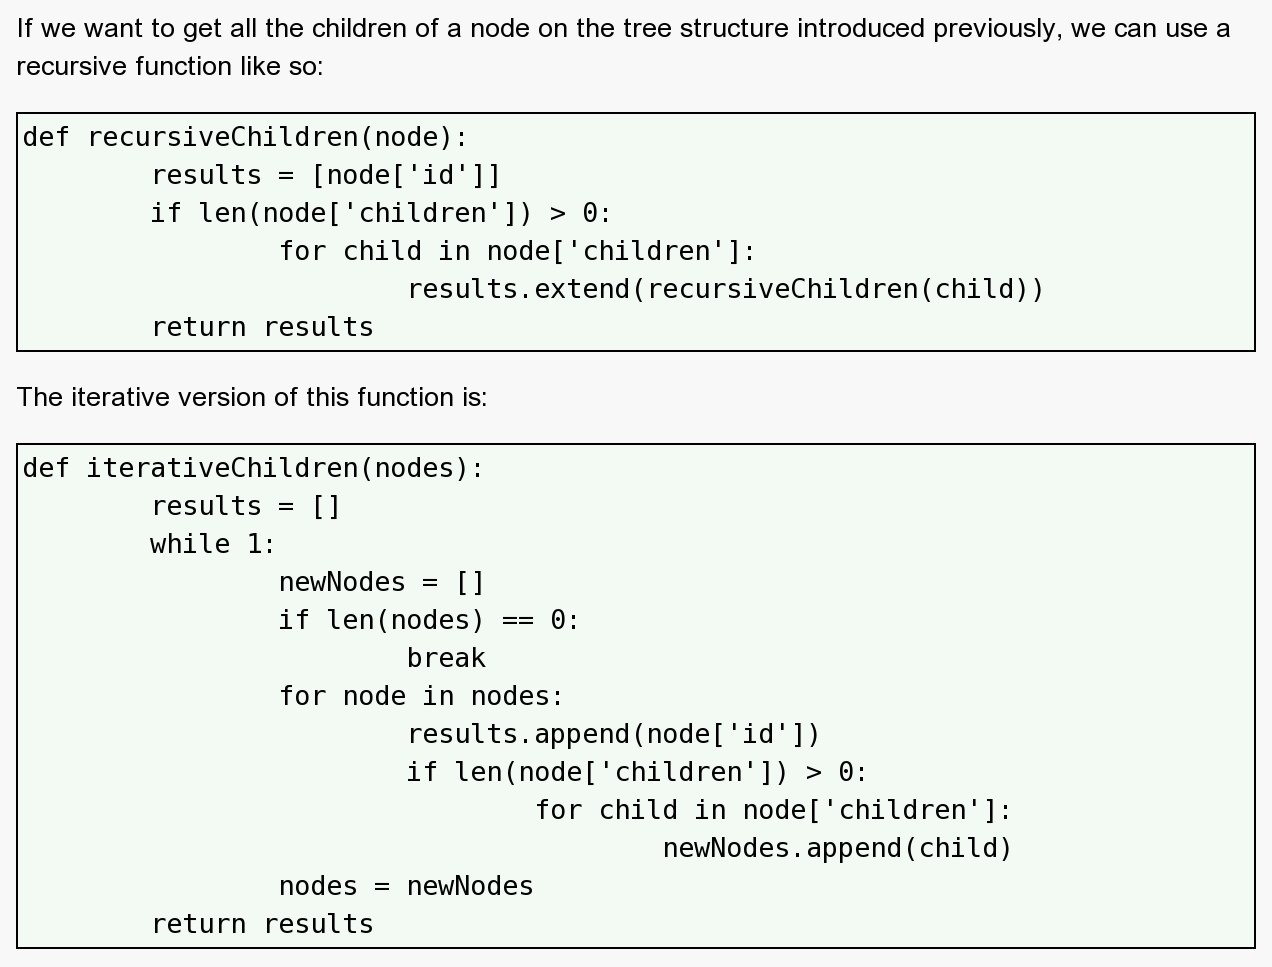
\includegraphics[scale=0.16]{pictures/recursive_vs_iteractive.png}
  \end{center}
}

\frame {
  \frametitle{Пример}

  Написать функцию f(n), которая вернёт сумму арифметической прогрессии

  \vspace{0.5cm}
  $1 + 2 + 3 + ... + (n - 1) + n$
}

\begin{frame}[fragile]
  \frametitle{Итерационный алгоритм}
  \begin{minted}{java}
static int f(int n) {
    int sum = 0;
    for (int i = 1; i <= n; i = i + 1) {
        sum = sum + i;
    }
    return sum;
}
  \end{minted}
\end{frame}

\begin{frame}[fragile]
  \frametitle{Итерационный алгоритм 2}
  \begin{minted}{java}
static int f(int n) {
    int sum = 0;
    for (int i = n; i >= 1; i = i - 1) {
        sum = sum + i;
    }
    return sum;
}
  \end{minted}
\end{frame}

\begin{frame}[fragile]
  \frametitle{Итерационный алгоритм 3}
  \begin{minted}{java}
static int f(int n) { // аргументы функции - тоже
                      // локальные переменные
    int sum = 0;
    while (n >= 1) {
        sum = sum + n;
        n = n - 1;    // их тоже можно менять
    }
    return sum;
}
  \end{minted}
\end{frame}

\begin{frame}[fragile]
  \frametitle{Рекурсивный алгоритм}
  \begin{minted}{java}
static int f(int n) {
    if (n <= 1) {
        return 1;
    } else {
        return n + f(n - 1);
    }
}
  \end{minted}
\end{frame}

\frame {
  \frametitle{Риск переполнения стека вызовов (Call Stack Overflow)}
  Мы рассмотрели простой случай \underline{не хвостовой} рекурсии

  \vspace{0.5cm}
  \underline{Не хвостовые} рекурсии \underline{не оптимизируются} трансляторами в \underline{итерационные алгоритмы}\footnote{В большинстве случаев}

  \vspace{0.5cm}
  При большом числе вызовов \underline{можно получить crash}, известный как <<переполнения стека>>
}

\frame {
  \frametitle{Как избежать stack overflow?}
  \begin{itemize}
    \item убедиться, что функция \underline{вызывает себя небольшое количество раз} (и уж точно не бесконечное число раз)
    \item если функция должна вызывать себя много раз (например обойти все/значительное количество элементов массива) --- убедиться, что рекурсивный вызов \underline{хвостовой}
    \item есть и другие нюансы, в зависимости от языка и выбранного уровня оптимизации транслятора
  \end{itemize}
}

\begin{frame}[fragile]
  \frametitle{Не хвостовая рекурсия}
  Если функция идет по ветке, где должна вызвать себя, но \underline{перед возвратом/выходом} она делает что-то \underline{отличное от вызова самой себя} --- она \textbf{не хвостовая}

  \vspace{0.5cm}
  Не хвостовой вызов (последнее действие --- сложение)
  \begin{minted}{python}
return n + f(n - 1)
  \end{minted}

  \vspace{0.5cm}
Более подробная версия этого кода:
  \begin{minted}{python}
a = n - 1
b = f(a)          # (1)
c = n + b         # (2)
return c
  \end{minted}

  \vspace{0.5cm}
  Строки (1) и (2) местами не поменяешь
\end{frame}

\begin{frame}[fragile]
  \frametitle{Хвостовая рекурсия}
  \begin{minted}{java}
static int f(int n, int sum = 0) { // значение аргумента
                                   // по-умолчанию
    if (n <= 0) {
        return sum;
    } else {
        return f(n - 1, sum + n);  // последним будет
                                   // выполнен вызов
                                   // функции f
    }
}
  \end{minted}
\end{frame}

\frame {
  \frametitle{Неявная рекурсия}

  Мы рассмотрели случаи с \underline{явной рекурсией}, когда \underline{из кода функции} видно, что она \underline{вызывает себя}

  \vspace{0.5cm}
  Но возможна и следующая ситуация:
  \begin{itemize}
    \item функция A вызывает функцию B
    \item функция B вызывает функцию A
  \end{itemize}

  В этом случае функция A называется \underline{неявно рекурсивной}
}

\end{document}
